\documentclass[a4paper]{article}
\usepackage{placeins}
\usepackage{pdfpages}
\usepackage{graphicx}
\usepackage{float}
\usepackage{gensymb}
\usepackage{listings}
\usepackage{color} %red, green, blue, yellow, cyan, magenta, black, white
\definecolor{mygreen}{RGB}{28,172,0} % color values Red, Green, Blue
\definecolor{mylilas}{RGB}{170,55,241}

\renewcommand{\thesubsection}{\thesection.\alph{subsection}}

\lstset{language=Matlab,%
	%basicstyle=\color{red},
	breaklines=true,%
	morekeywords={matlab2tikz},
	keywordstyle=\color{blue},%
	morekeywords=[2]{1}, keywordstyle=[2]{\color{black}},
	identifierstyle=\color{black},%
	stringstyle=\color{mylilas},
	commentstyle=\color{mygreen},%
	showstringspaces=false,%without this there will be a symbol in the places where there is a space
	numbers=left,%
	numberstyle={\tiny \color{black}},% size of the numbers
	numbersep=9pt, % this defines how far the numbers are from the text
	emph=[1]{for,end,break},emphstyle=[1]\color{red}, %some words to emphasise
	%emph=[2]{word1,word2}, emphstyle=[2]{style},    
}

\title{Assignment 2: Mini project\\
	\large Environmental monitoring from satellite}
\author{Toke Frederiksen}
\date{\today}


\begin{document}

\maketitle
	
\section{Mr X's potatoes}
\subsection*{Part 1a}
The given data is presented as an RGB image in figure \textbf{FIGUREEKJDEKJDEJK}. The Ihh intensity was used as the red channel, Ihv as green and Ivv as blue. Further the values are presented in dB and have been conned to values between 0 and 1. The MATLAB code can be found in assignment2 1.m, part 1a. The ground truth map is presented in figure \textbf{IFURIREG}, in colours according to the corresponding colour map. It shows the class of each pixel by its colour code.
\begin{figure}[ht]
	\centering
		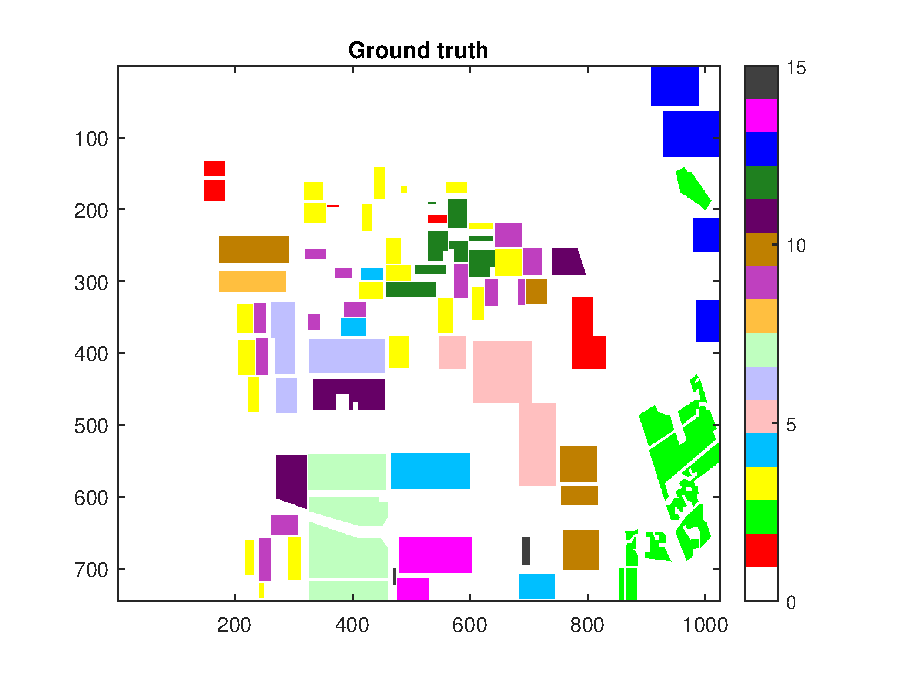
\includegraphics[width=1\textwidth
		]{gtruth}
		\caption{text}\label{key}
\end{figure}

\subsection*{Part 1b}
The code for this part can be found in splitData.m and assignment2_1.m. The data, ie. each class from 1-15, is split into 60 \% test set and 40 \% training set. It is done by a random permutation of the pixels in each class, and then selecting the first 69 \% for the test set and the remaining for the training data.

\subsection*{Part 1c}
A histogram of the $ I_{HH} $, $ I_{HV} $ and $ I_{VV} $ channel for all pixels in class 5 (potato) is shown in figure \textbf{REFEFE}, along with the gamma function for the respective channel. As seen from the figure, the gamma function describes the histogram well, except for the $ I_{HV} $ channel. 

\section{San Francico needs your help}




\end{document}